\documentclass{article}
\usepackage[utf8]{inputenc}
\usepackage[spanish]{babel}
\usepackage{listings}
\usepackage{graphicx}
\graphicspath{ {images/} }
\usepackage{cite}

\begin{document}

\begin{titlepage}
    \begin{center}
        \vspace*{1cm}
            
        \Huge
        \textbf{Taller - Nociones de la memoria del computador}
            
        \vspace{1.5cm}
        
        \textbf{Diego Andrés Zuluaga Alzate}
        
        \vspace{1.5cm}
        
        \begin{figure}[h]
        
\includegraphics[width=6cm]{logoudea.png}
        \centering
        \label{fig:logoudea}
        \end{figure}
            
        \vspace{0.7cm}
            
        \Large
        Universidad de Antioquia\\
        Medellín\\
        Septiembre de 2020
            
    \end{center}
\end{titlepage}

\tableofcontents

\break

\section{La memoria del computador}
¿Qué es la memoria del computador?, es una pregunta frecuente que nos hacemos en la cotidianidad, sabemos que esta allí para que el computador pueda funcionar pero no sabemos mucho más, ¿entonces que podemos decir sobre la memoria?, pues esta es la encargada de almacenar información durante un periodo de tiempo, dispuesta allí porque se le dio una tarea a cumplir al microprocesador, la memoria guarda temporalmente esa información u orden que le demos al equipo y al acabar con el proceso  la información vuelve a su lugar original  y es borrada de la memoria para que no ocupe espacio algo que ya ha sido utilizado.\cite{memoria}
 
 \vspace{0.4cm}

\section{Los tipos de memoria} 

\vspace{0.3cm}

\subsection{Memoria cache L1,L2,L3}

La memoria cache es más rápida que la memoria RAM a costa de tener menos capacidad que la antes dicha, la cache guarda información que es usada frecuentemente para su rápido acceso. En L1 se guardan instrucciones además de frecuentes importantes ya que es la más rápida al encontrarse en el núcleo del microprocesador, L2 y L3 son un poco más lentas pero también con más capacidad, pueden contener la misma información que el nivel que lo precede y tambien información adicional.

\vspace{0.3cm}

\subsection{memoria RAM}

La memoria RAM es en lo primero que piensas cuando te mencionan la memoria de un computador, en ella se almacena la mayoria de informacion temporal del equipo, por su facil acceso y gran capacidad.

\vspace{0.6cm}

A continuación se presenta una memoria RAM comun (\ref{fig:RAM})

\begin{figure}[h]
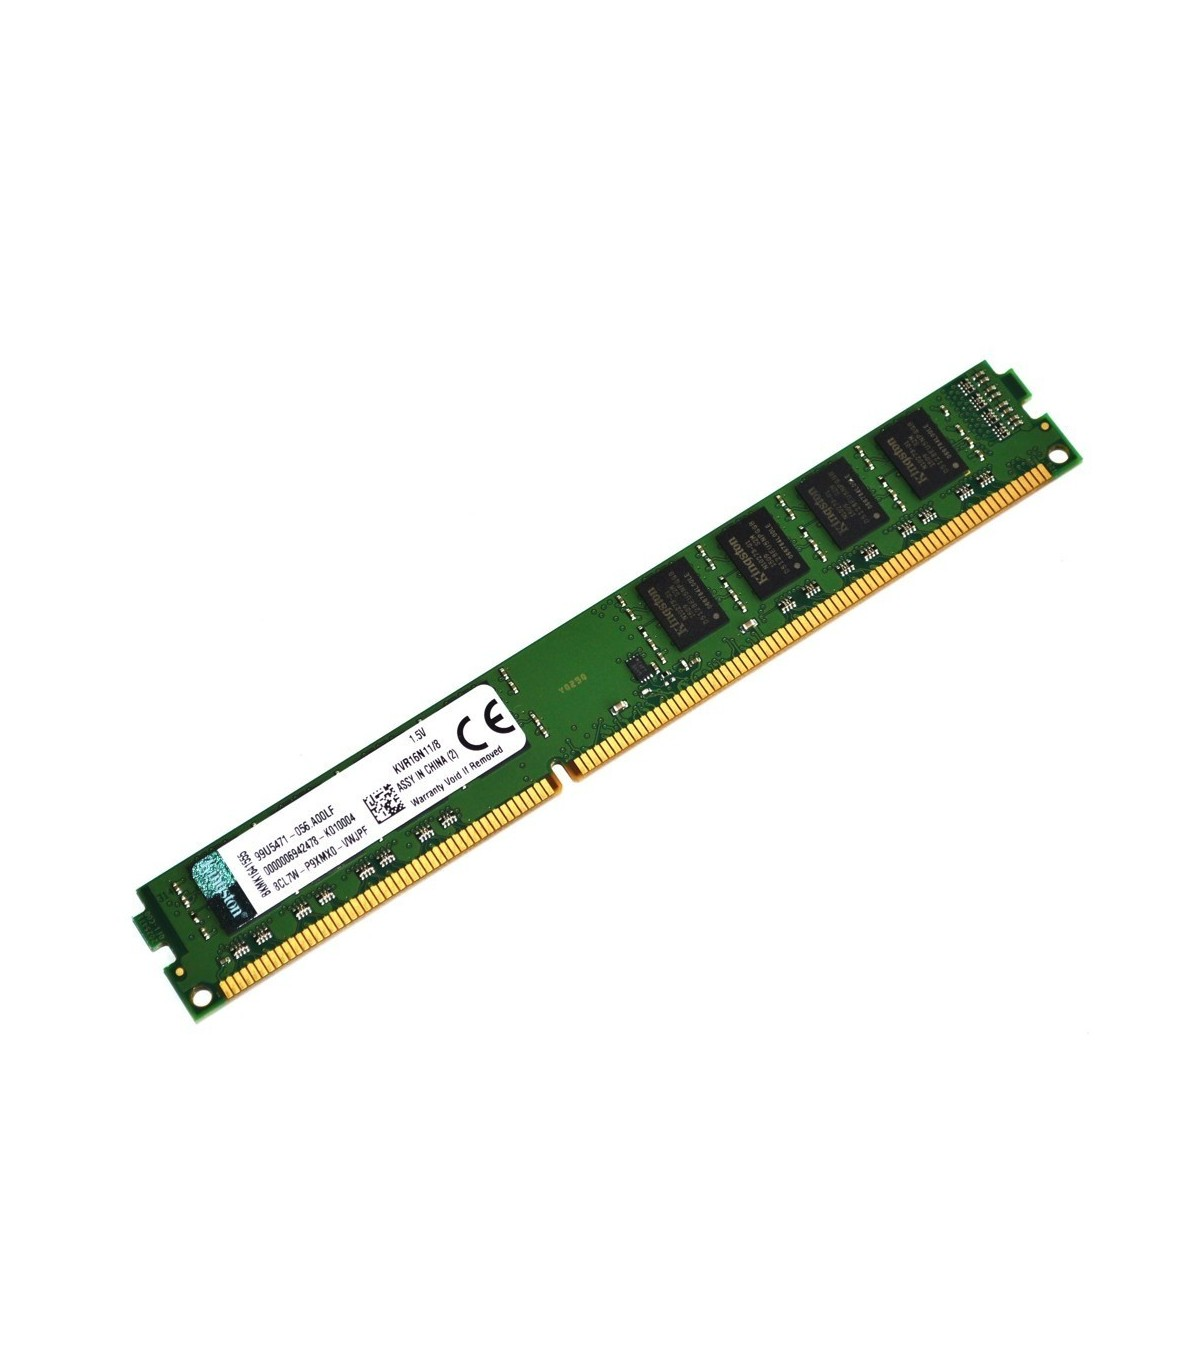
\includegraphics[width=4cm]{RAM.jpg}
\centering
\caption{Memoria RAM}
\label{fig:RAM}
\end{figure}

\vspace{0.3cm}

\subsection{memoria Virtual}

La memoria virtual es una porción del disco duro dedicada a guardar pedazos de información de algún programa o tarea que se está procesando pero que son muy poco utilizados o que ocupan espacio innecesario en el momento, y es mejor tenerlos separados para que se puedan llamar cuando el proceso en ejecución lo requiera.

\vspace{0.3cm}

\subsection{Disco Duro}

El disco duro es la memoria con más capacidad de almacenamiento, pero también es la más lenta, acceder a la información se limita a la velocidad de rotación de los discos que contiene.

\vspace{0.6cm}

A continuación se presenta una Dico Duro comun (\ref{fig:discoduro})

\begin{figure}[h]
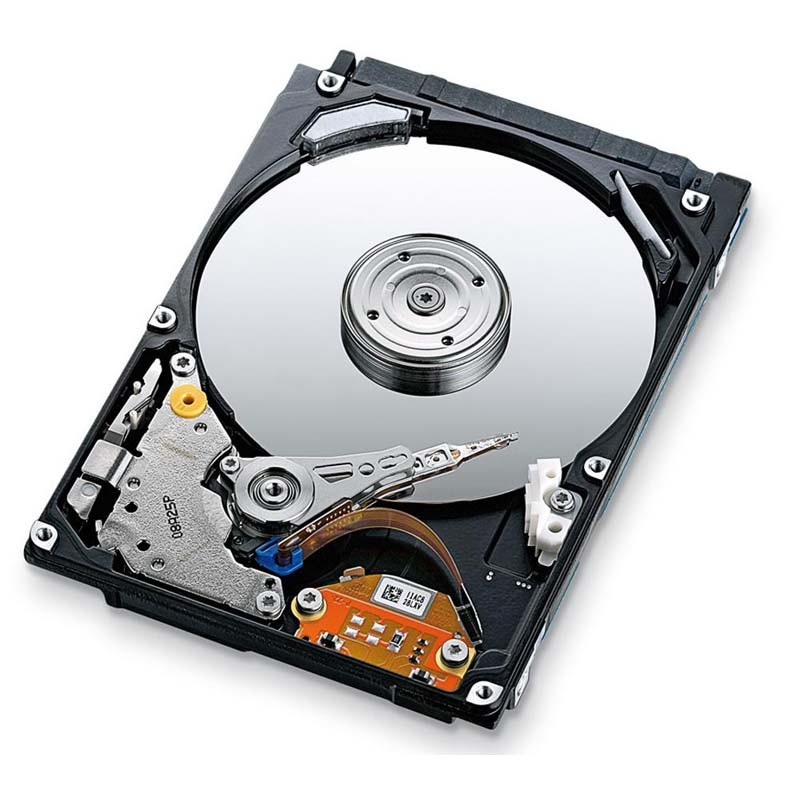
\includegraphics[width=4cm]{discoduro.png}
\centering
\caption{Disco Duro}
\label{fig:discoduro}
\end{figure}

\section{Gestión de la memoria en una computadora} 

En la gestión de memoria se separan las direcciones físicas donde está la información en unas nuevas direcciones virtuales para mejorar el rendimiento de la RAM, para poder lograr esto lo que pasa es que se traslada la información que debe ser ejecutada por el procesador a la memoria virtual por medio de dos técnicas.

Partición fija: donde el usuario separa en varias partes de igual o diferente tamaño

Partición dinámica: en esta partición dependiendo de la cantidad de memoria que necesite cada proceso estos tamaños se ajustaran. 

\vspace{0.6cm}

\section{velocidad de la memoria}

\vspace{0.3cm}

\subsection{¿Qué hace que una memoria sea más rápida que otra?}

Lo que hace más rápida una memoria determinada es la facilidad que tenga el procesador de acceder a la información contenida en ella, por eso en el caso de la memoria cache y la RAM donde la información es temporal, pero se puede acceder a ella de una forma muy fácil esto las hace más eficientes que un disco duro.

\vspace{0.3cm}

\subsection{¿Por qué esto es importante?}

acceder a la información rápidamente hace que el equipo pueda ejecutar ordenes sin ningún problema, no nos tenemos que preocupar por los lapsos de espera.

\bibliographystyle{IEEEtran}
\bibliography{references}

\end{document}
